\documentclass{sig-alternate}

\usepackage{graphicx} 
\usepackage{subfigure}
\usepackage{paralist}

\usepackage{hyperref}

\usepackage{url}
\usepackage{booktabs}

\usepackage[usenames,dvipsnames]{xcolor}
\usepackage{tikz}
\usetikzlibrary{positioning, calc}

\usepackage[draft,nomargin,footnote]{fixme}

\graphicspath{{figs/}}

\usepackage{xspace}
\newcommand{\eg}{\textit{e.g.}\xspace}
\newcommand{\etal}{\textit{et al.}\xspace}
\newcommand{\ie}{\textit{i.e.}\xspace}
\newcommand{\etc}{\textit{etc.}\xspace}
\newcommand{\vs}{\textit{vs.}\xspace}

\begin{document}

% if need info about conference :
%\conferenceinfo{WOODSTOCK}{'97 El Paso, Texas USA}

\title{CoWriter : Two case Studies}


\author{Alexis Jacq$^{1,2}$, S\'everin Lemaignan$^1$, Fernando Garcia$^1$, Ana Paiva$^2$, Pierre Dillenbourg$^1$ \\
$^1$CHILI Lab, \'Ecole Polytechnique F\'ed\'erale de Lausanne, Suisse,\\
$^2$Instituto Superior T\'{e}cnico, University of Lisbon, Portugal}


%   \author{
%   % 1st. author
%   \alignauthor
%   Alexis Jacq\\
%       \affaddr{EPFL}\\
%       \affaddr{IST}
%   % 2nd. author
%   \alignauthor
%   Severin Lemaignan\\
%       \affaddr{EPFL}
%   \and
%   % 3rd. author
%   \alignauthor Fernando Garcia\\
%       \affaddr{EPFL}
%
%   \alignauthor Pierre Dillembourg\\
%       \affaddr{EPFL}
%
%   \alignauthor Ana Paiva\\
%           \affaddr{IST}
%    }


\date{date comes here}


\maketitle
\begin{abstract}
Abstract comes here
\end{abstract}

\keywords{robot-supported educative activitiy, handwriting learning, learning
by teaching}

\section{Introduction}
% -> A new hri field
% -> What as been done before
% -> what is new here

%   \begin{figure}
%       \centering
%       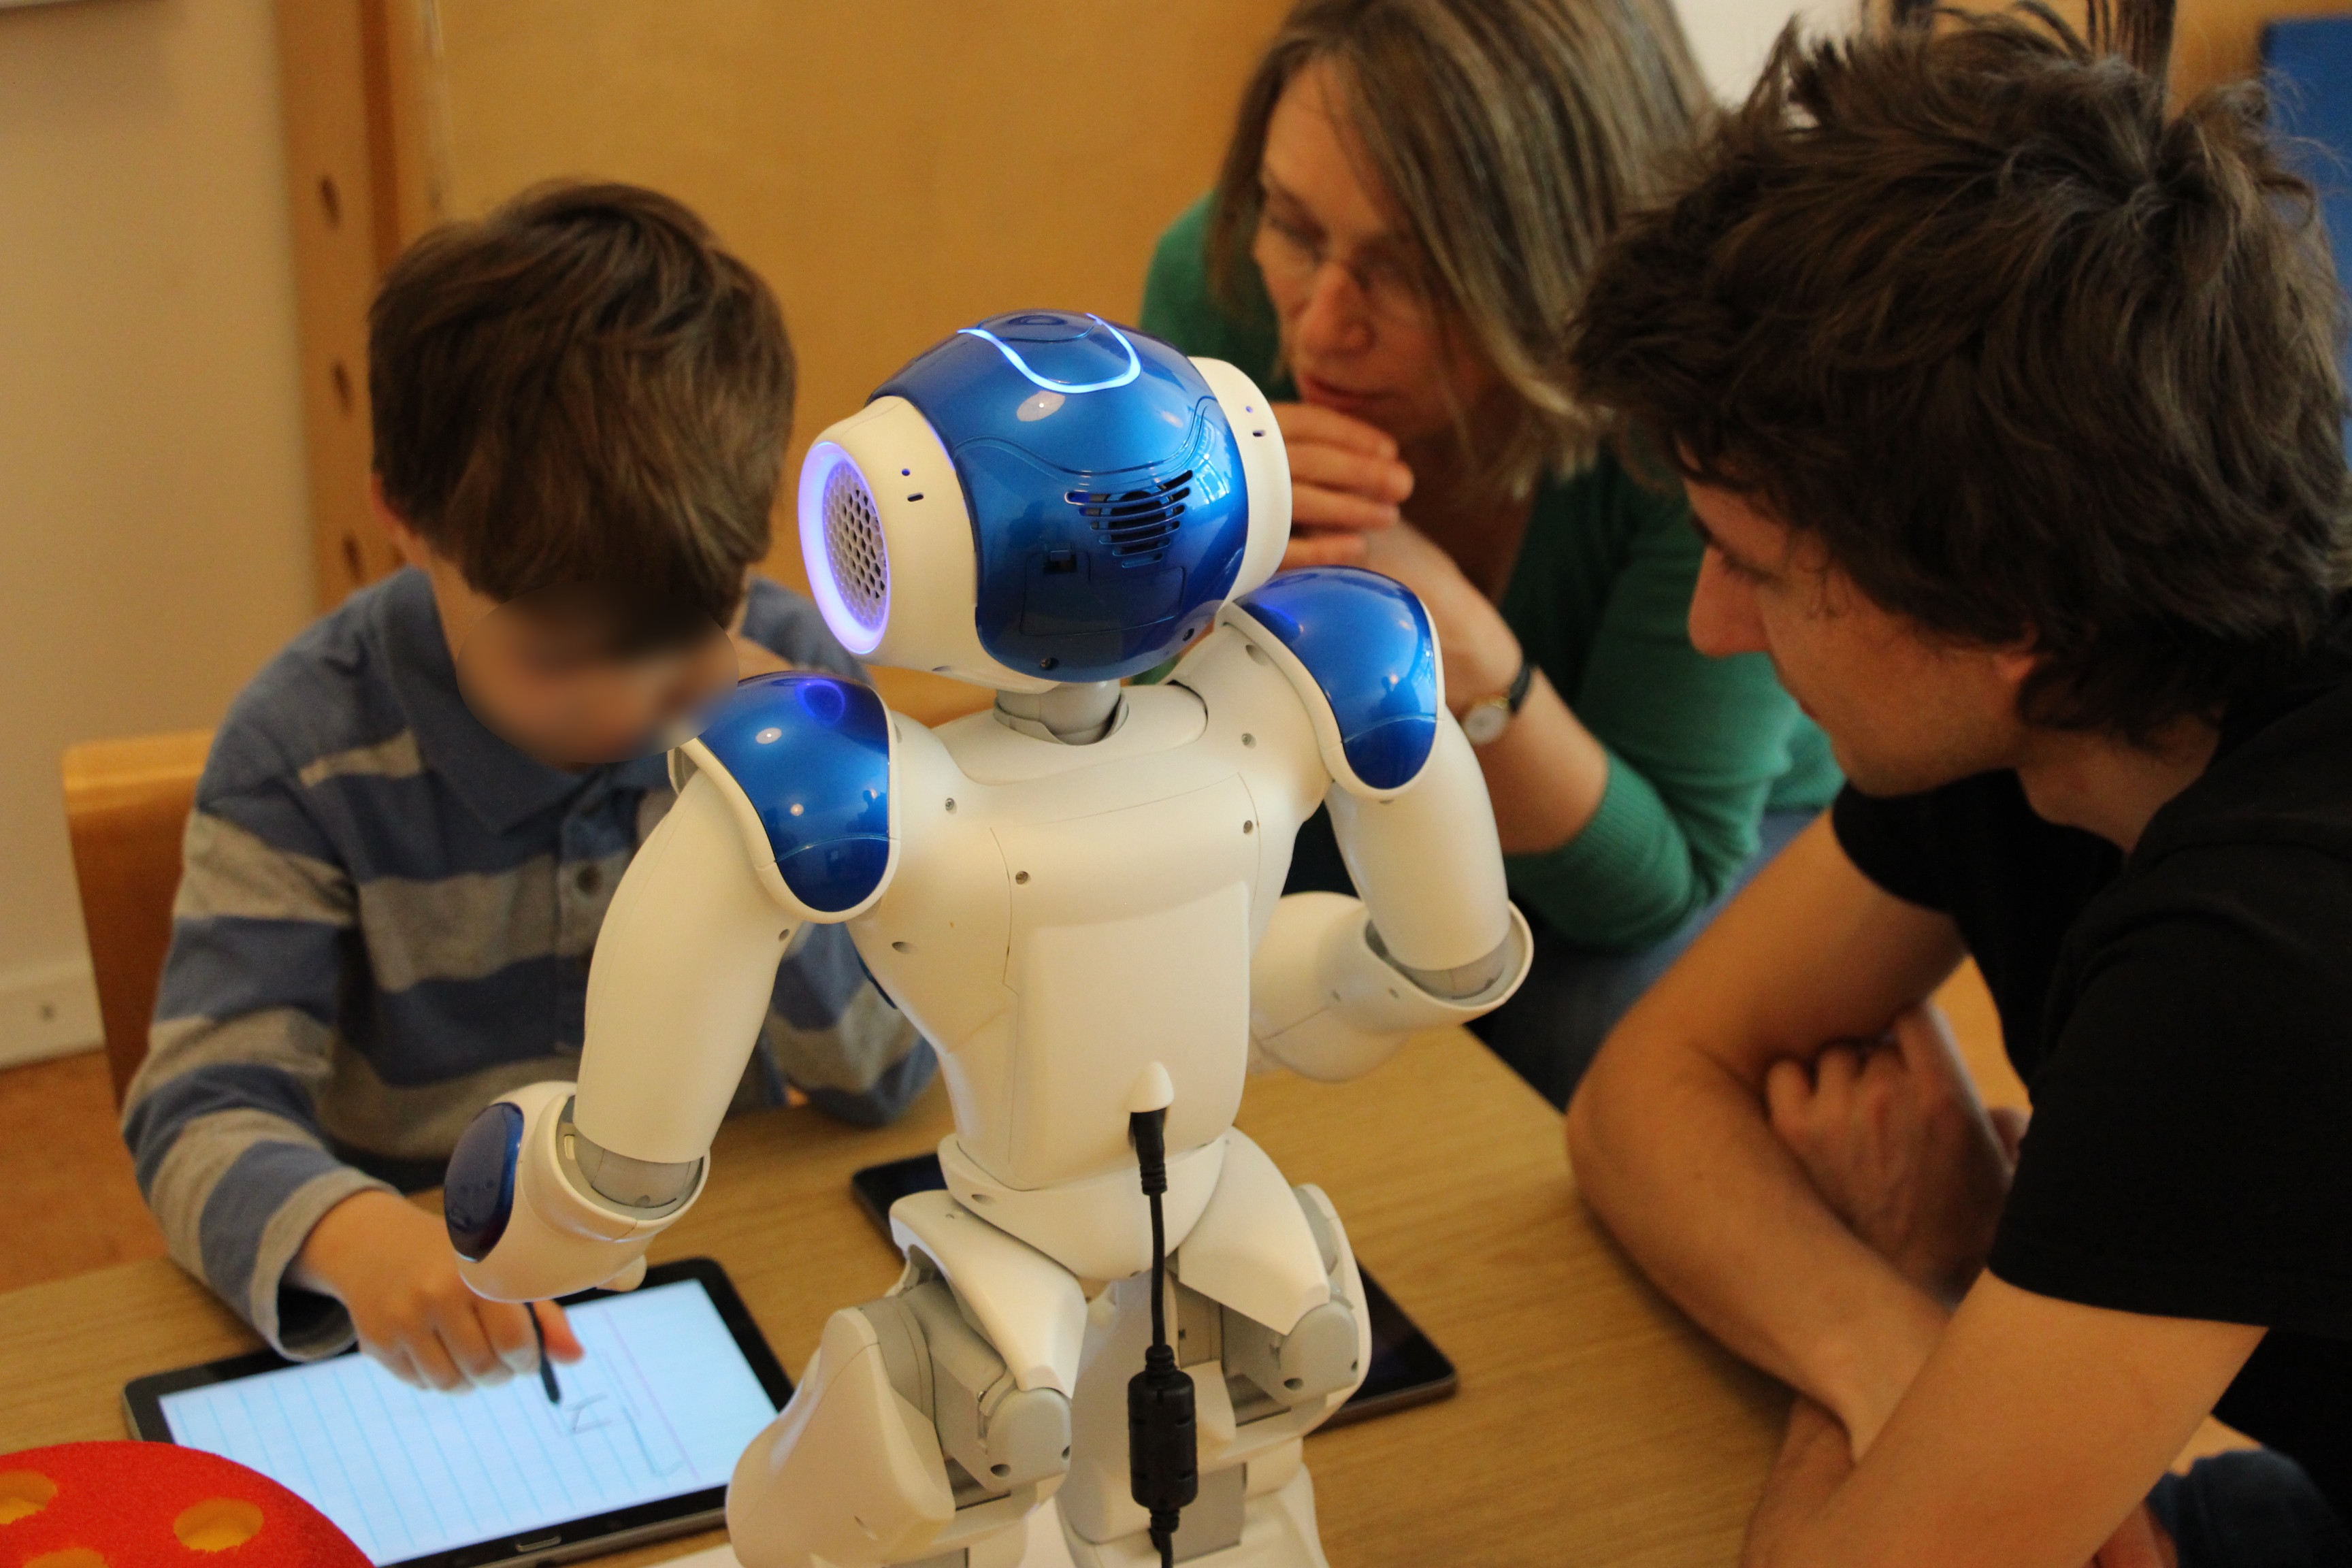
\includegraphics[width=0.9\linewidth]{henry}
%       \caption{Henry teaching Nao how to write numbers, with the help of an occupational therapist.}
%       \label{fig:henry}
%   \end{figure}

\section{The CoWriter activity}
\subsection{Children teach handwriting to the robot}
\subsection{Our approach}

\subsection{Learning and generating letters}

\subsection{robotic implementation}

\section{case 1 : Diego}
\subsection{Context}
Diego is a five years old child. Her mother told us he had difficulties to learn
writing at school, particulary in drawing cursive letters. Before experiments,
she provided us with a homework of Diego to show explicitly his handrwiting
level (fig). 

From our perspective, Diego is shy and quiet. He suffers from a poor
self-esteam much more than any actual trouble in writing.

\subsection{Questions}
The CoWriter activity needs a child engaged as interaction leader. 
In this study we consider the problem of long-term interactions : is it possible to
sustain this engagement over several one-hour sessions ?

%   \begin{figure}
%       \centering
%       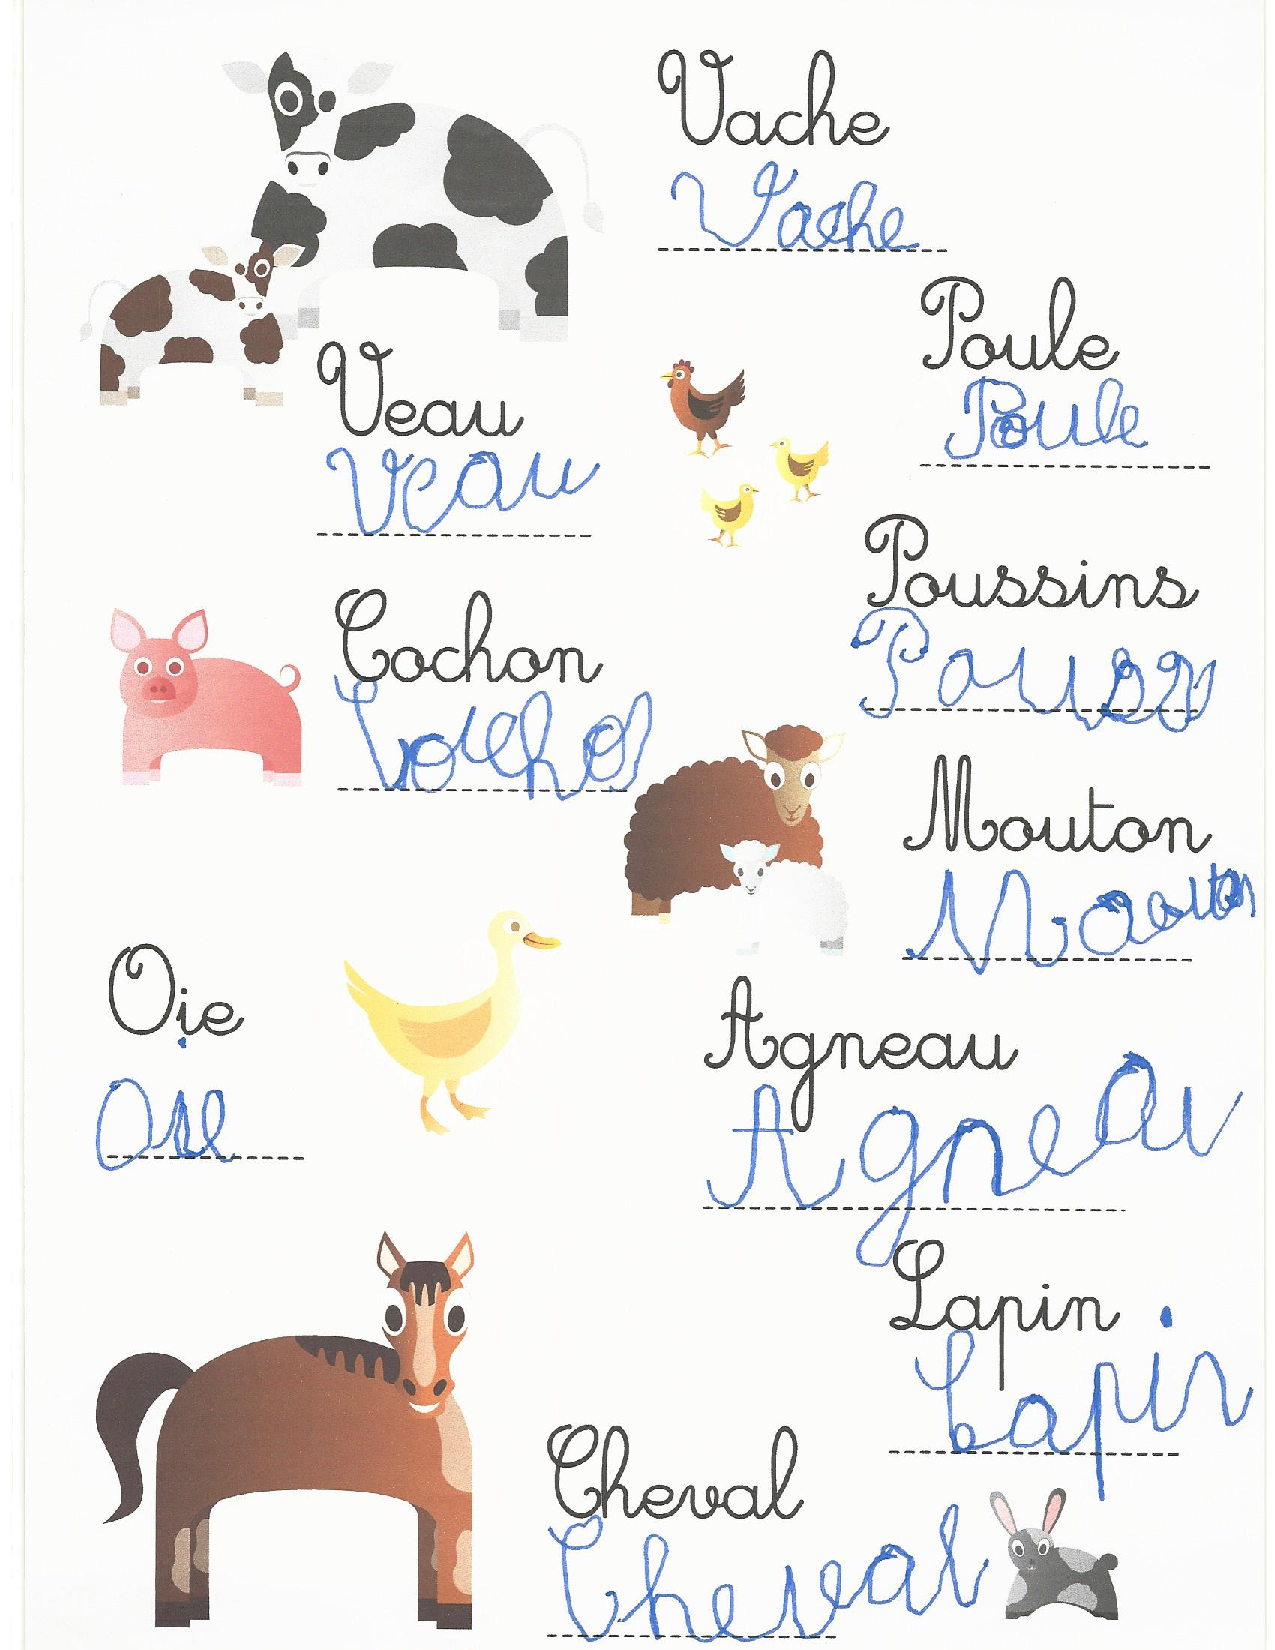
\includegraphics[width=0.9\linewidth]{diego_start}
%       \caption{Homework performed by Diego before the experiment. It gives an
%       overvew of his starting level in handwriting.}
%       \label{fig:diego_start}
%   \end{figure}

%   \begin{figure}
%       \centering
%       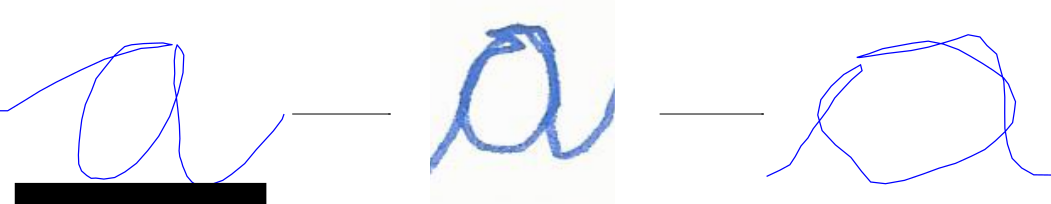
\includegraphics[width=0.9\linewidth]{3a}
%       \caption{Letter deformation along an eigenvector. \emph{Left} : the non-deformed
%           letter (origin of the eigenspace). \emph{Middle} : the actual Diego's
%           deformation (from figure~\ref{fig:diego_start}). \emph{Right} : exaggerated
%   deformation along the eigenvector that encode Diego's mistake.} 
%       \label{fig:3a}
%   \end{figure}

\subsection{Experimental settings}

The experiment took place in our laboratory. Our goal was to figure out 
an environment in order to make Diego sustaining
engagement over four sessions of one hour, one session per week. We decided 
to introduce an appealing scenario that justifyed to the child the activity 
where a robot wants to learn handwriting. We used two Nao robots : a blue one 
(called Mimi) and an orange one (called Clem). Mimi was away for a 
scientific mission, and the two robots had to communicate by mails. But they decided to do it 
``like humans", with handwritten messages. While Mimi was good in handwriting, 
Clem had strong difficulties and needed the help of Diego.

The mission of Mimi consisted in the exploration of a mysterious hidden
base. Each week, just before the session, it was sending a postal mail contening
a picture, a curious object it found and a few handwritten words about its discoveries. 
The pictures was representing itself exploring 
a dark room of the hidden base (that was actually our laboratory's workshop). 
The objects where 3D printed. In fact, there where puzzle pieces of a small 3D 
model of Nao robot but regarding them one by one, it was not easy to guess it.

During the three first session, Clem (the other robot) was waiting for Diego
with the recieved mail. It let Diego take a look to the picture and the object,
and then it asked him to read the message.
Finaly, Diego figured out a response and helped the robot to write it.

The fourth and last session was set as a test: Mimi, the ``explorer'' robot,
had come back from its mission and it actually challenged Clem in
front of Diego: \emph{``I don't believe you wrote yourself these nice letters that I
received! Prove it to me by writing something in front of me!''} This situation
was meant to evidence the Prot\'eg\'e effect: by judging the other robot's
handwriting, Mimi would implicitly judge Diego's skills as
teacher, and in turn, Diego's handwriting.

% -> level increase
% -> lettres en plastic

%   \begin{figure}
%       \centering
%       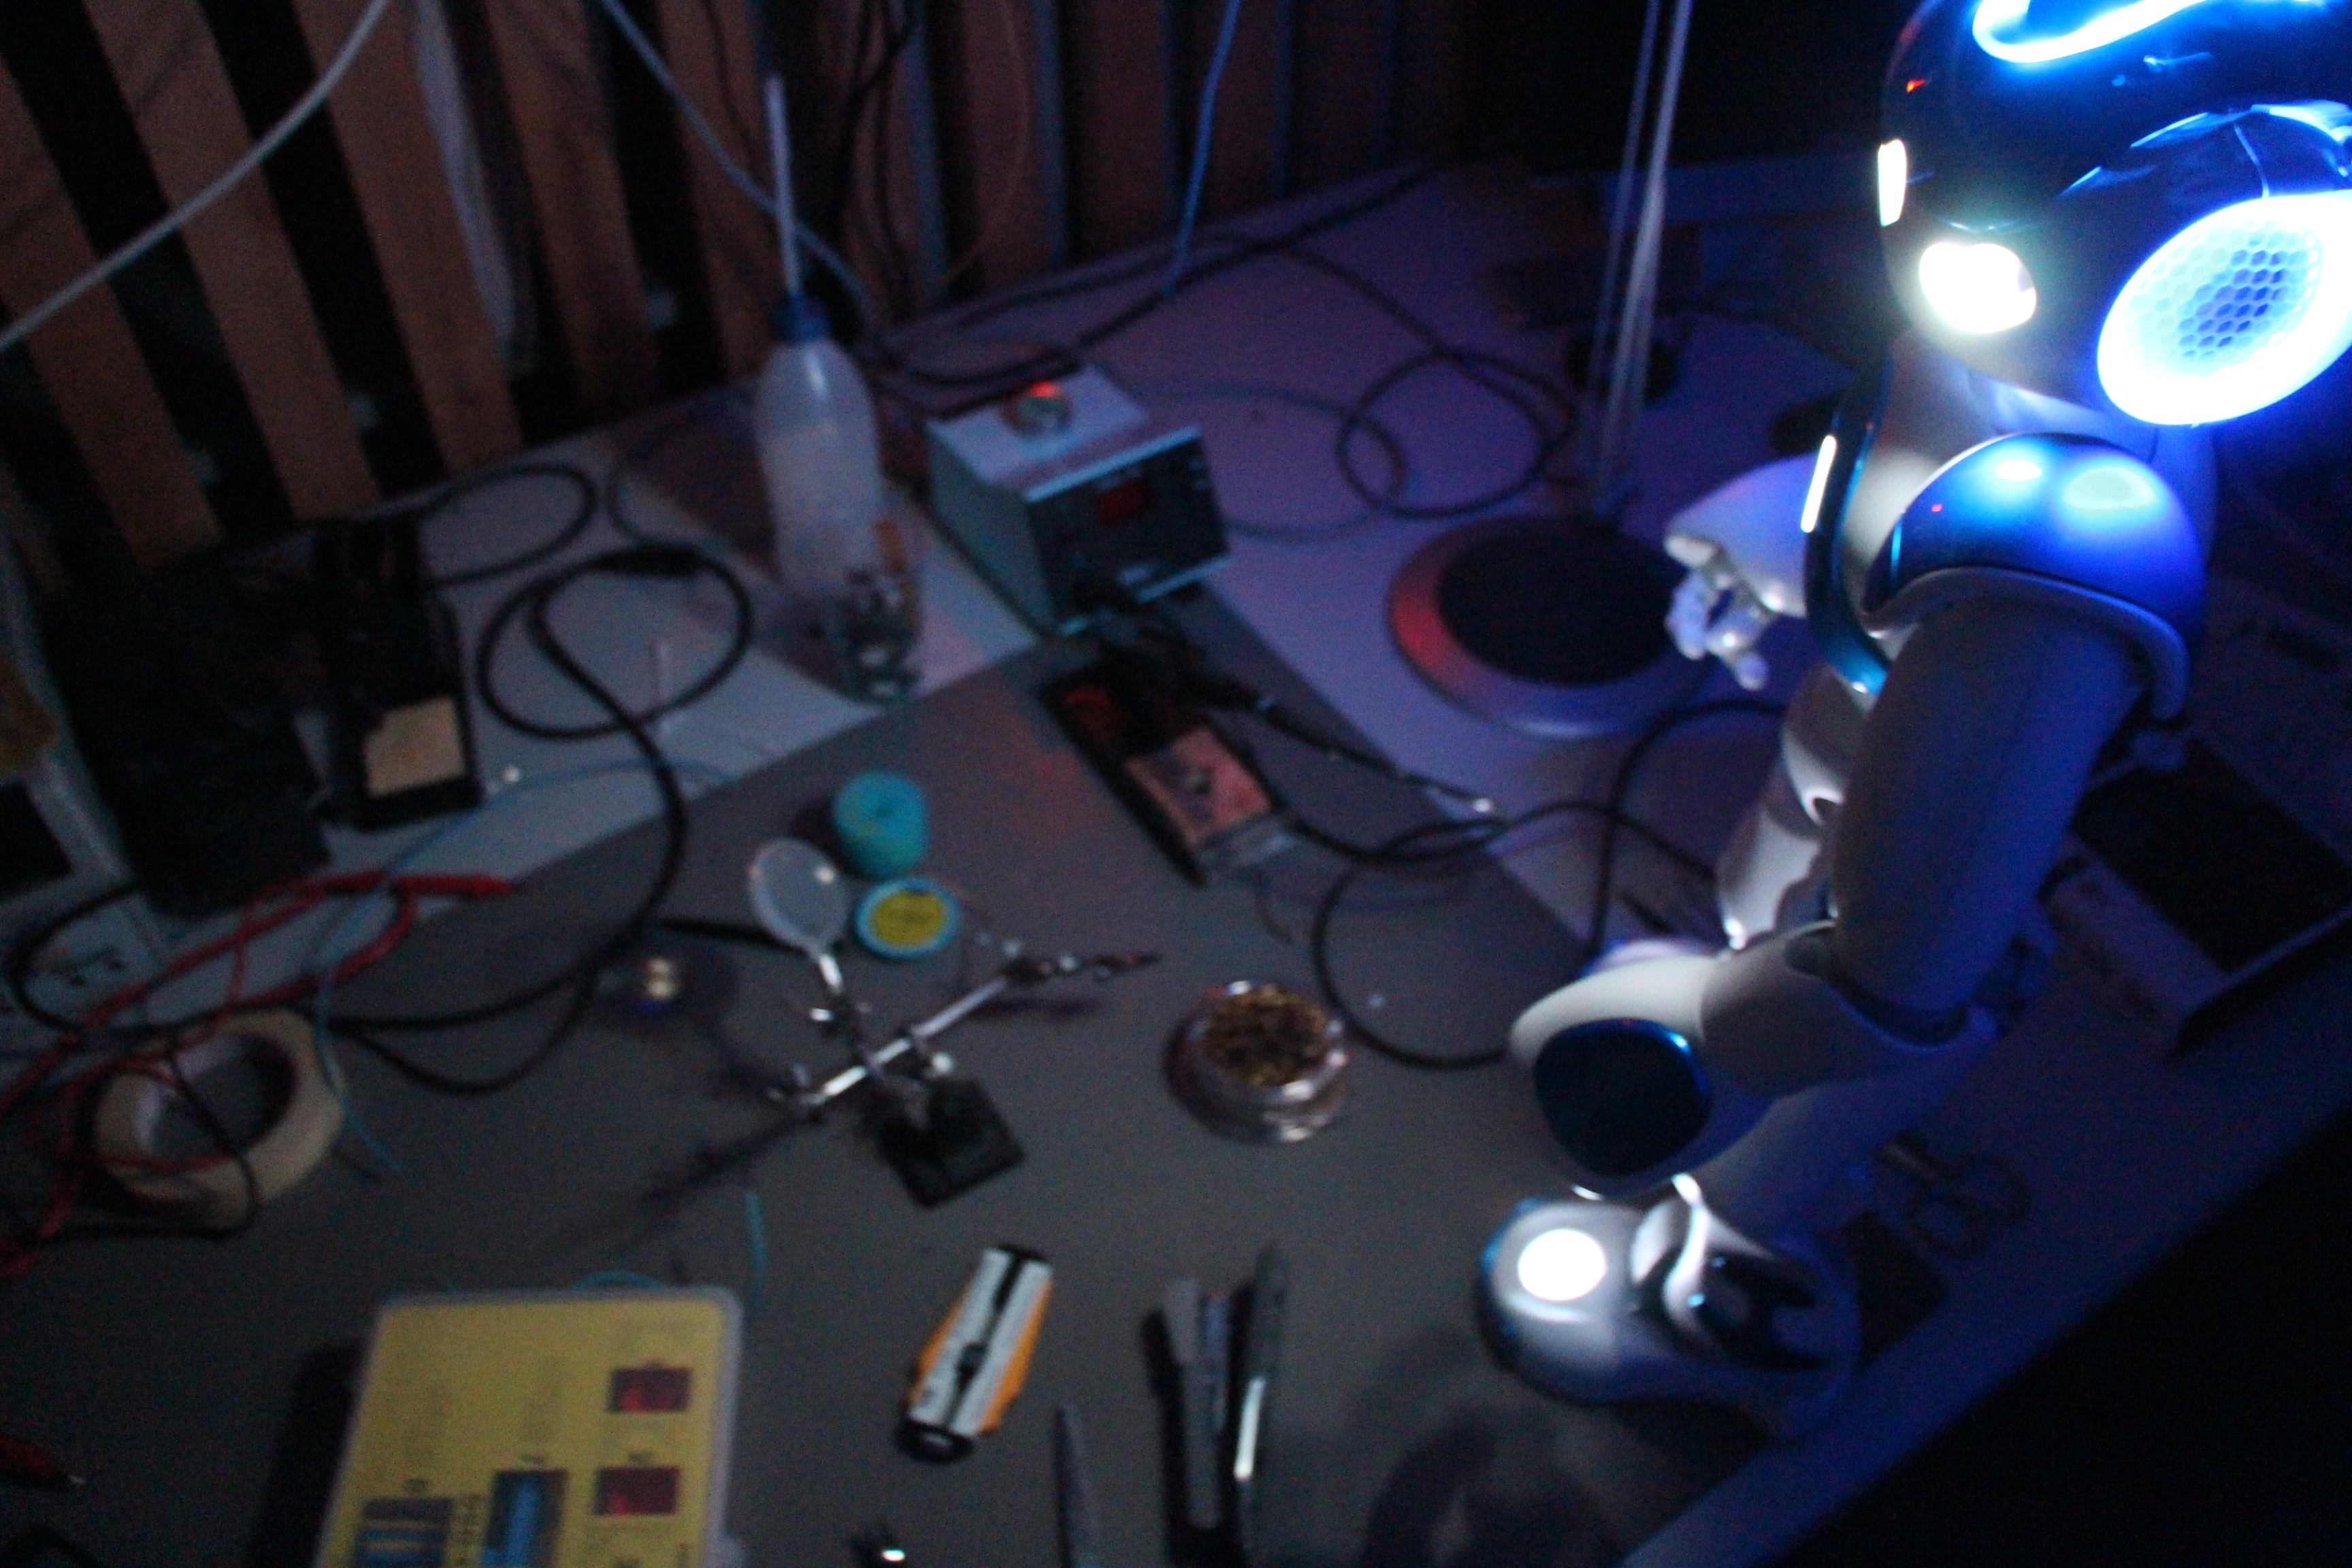
\includegraphics[width=0.9\linewidth]{mimi_mails}
%       \caption{Exemple of content of the mails sent by Mimi. A : pictures of Mimi exploring the
%           hidden base. B : some curious objects found by Mimi in the base. C :
%           few words about its adventures and discoveries.
%       }
%       \label{fig:mimi_mails}
%   \end{figure}


\subsection{Results}

\section{case 2 : Henry}
Description of experiments \& results with Diego

\subsection{Experiment design}

\subsection{Results}

\section{Discussion}

\section{Conclusions}

\bibliographystyle{abbrv}
\bibliography{cowriter} 
\end{document}
